\section{}
\[
H(s)=\frac{4}{s^2-4}=\frac{4}{(s-2)(s+2)}\,.
\]
\subsection{Bode-Diagramm}
\begin{center}
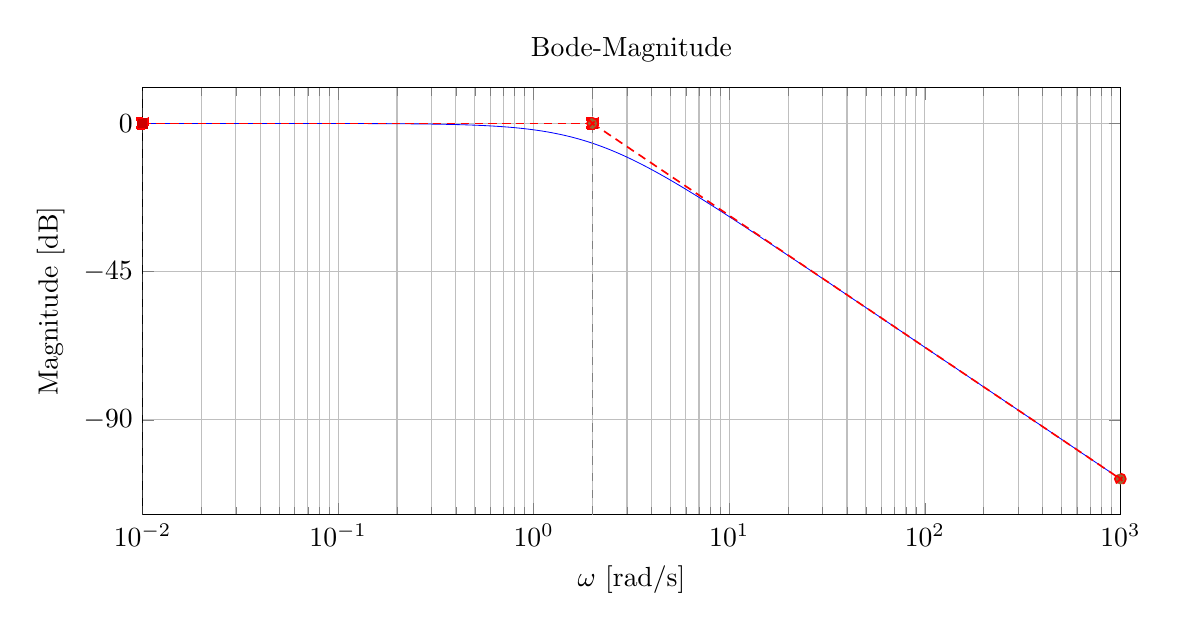
\begin{tikzpicture}
\begin{semilogxaxis}[
  width=14cm,height=7cm,
  xmin=1e-2,xmax=1e3,
  xlabel={$\omega$ [rad/s]},
  ytick distance=45,
  ylabel={Magnitude [dB]},
  grid=both,
  title={Bode-Magnitude}
]
\addplot[
  domain=1e-2:1e3,
  samples=800,
  mark=none,
  line width=0.3pt,
  blue
] {-40*ln(sqrt(1 + (x/2)^2))/ln(10)};
\addplot+[domain=1e-2:2,samples=2,dashed,dash pattern=on 3pt off 2pt,line width=0.6pt,red] {0};
\addplot+[domain=2:1e3,samples=2,dashed,dash pattern=on 3pt off 2pt,line width=0.6pt,red] {-40*ln(x/2)/ln(10)};
\draw[gray,dashed] (rel axis cs:0,0) -- (rel axis cs:0,1);
\draw[gray,dashed] (axis cs:2,\pgfkeysvalueof{/pgfplots/ymin}) -- (axis cs:2,\pgfkeysvalueof{/pgfplots/ymax});
\node[gray,anchor=south east] at (axis cs:2,\pgfkeysvalueof{/pgfplots/ymax}) {\scriptsize Pole $\omega_p=2$ (LHP \& RHP)};
\end{semilogxaxis}
\end{tikzpicture}
\vspace{6mm}
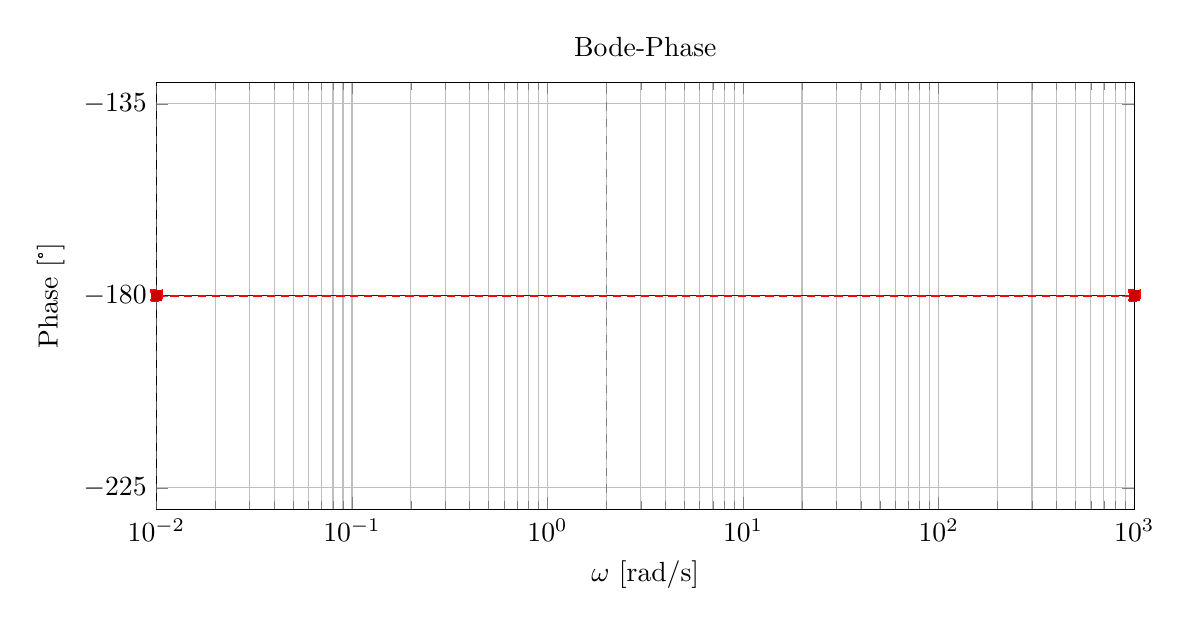
\begin{tikzpicture}
\begin{semilogxaxis}[
  width=14cm,height=7cm,
  xmin=1e-2,xmax=1e3,
  ymin=-230,ymax=-130,
  ytick distance = 45,
  xlabel={$\omega$ [rad/s]},
  ylabel={Phase [°]},
  grid=both,
  title={Bode-Phase}
]
\addplot[
  domain=1e-2:1e3,
  samples=2,
  mark=none,
  line width=0.3pt,
  blue
] {-180};
\addplot+[domain=1e-2:1e3,samples=2,dashed,dash pattern=on 3pt off 2pt,line width=0.6pt,red] {-180};
\draw[gray,dashed] (rel axis cs:0,0) -- (rel axis cs:0,1);
\draw[gray,dashed] (axis cs:2,\pgfkeysvalueof{/pgfplots/ymin}) -- (axis cs:2,\pgfkeysvalueof{/pgfplots/ymax});
\node[gray,anchor=south east] at (axis cs:2,\pgfkeysvalueof{/pgfplots/ymax}) {\scriptsize Pole $\omega_p=2$ (LHP \& RHP)};
\end{semilogxaxis}
\end{tikzpicture}
\end{center}
\newpage
\subsection{Erklärung}
\vspace{5mm}
\begin{description}[leftmargin=1.2em,labelsep=.6em,font=\bfseries]
\item[Schritt 1] Faktorisierung: $H(s)=\dfrac{4}{(s-2)(s+2)}$. DC-Wert $H(0)=-1\Rightarrow |H|_{\mathrm{DC}}=0\,\mathrm{dB}$; das negative Vorzeichen liefert eine konstante Phase von $-180^\circ$. Anfangssteigung $0\,\mathrm{dB/dec}$.
\item[Schritt 2] Pole bei $\omega_p=2\,\mathrm{rad/s}$ (einer RHP, einer LHP): Magnitudenbeitrag entspricht einem Doppelpol bei $\omega=2$ $\Rightarrow$ ab $\omega=2$ Slope $-40\,\mathrm{dB/dec}$. Am Eckpunkt exakte Dämpfung $-20\log_{10}2\approx-6\,\mathrm{dB}$. Phasenverlauf: die entgegengesetzen Beiträge der LHP- und RHP-Polphase heben sich auf; netto bleibt die Phase für alle $\omega$ konstant $-180^\circ$.
\item[Schritt 3] Grenzverhalten: für $\omega\ll2$ bleibt $|H(\j\omega)|\approx1$; für $\omega\gg2$ folgt $|H(\j\omega)|_{\mathrm{dB}}\approx-40\log_{10}(\omega/2)$; die Phase bleibt über das gesamte Spektrum bei $-180^\circ$.
\end{description}

\vspace{0.5cm}
\medskip
\noindent\textbf{Stückweise Näherung}
\[
|H(\j\omega)|_{\mathrm{dB}}\approx
\begin{cases}
0,& \omega\ll2,\\[4pt]
-20\log_{10}2,& \omega=2,\\[4pt]
-40\log_{10}(\omega/2),& \omega\gg2,
\end{cases}
\qquad
\]
\newpage